\documentclass[a4paper,14pt]{article}
\usepackage{float}
\usepackage{extsizes}
\usepackage{amsmath}
\usepackage{amssymb}
\everymath{\displaystyle}
\usepackage{geometry}
\usepackage{fancyhdr}
\usepackage{multicol}
\usepackage{graphicx}
\usepackage[brazil]{babel}
\usepackage[shortlabels]{enumitem}
\usepackage{cancel}
\usepackage{textcomp}
\usepackage{array} % Para melhor formatação de tabelas
\usepackage{longtable}
\usepackage{booktabs}  % Para linhas horizontais mais bonitas
\usepackage{float}   % Para usar o modificador [H]
\usepackage{caption} % Para usar legendas em tabelas
\usepackage{tcolorbox}

\columnsep=2cm
\hoffset=0cm
\textwidth=8cm
\setlength{\columnseprule}{.1pt}
\setlength{\columnsep}{2cm}
\renewcommand{\headrulewidth}{0pt}
\geometry{top=1in, bottom=1in, left=0.7in, right=0.5in}

\pagestyle{fancy}
\fancyhf{}
\fancyfoot[C]{\thepage}

\begin{document}
	
	\noindent\textbf{6FMA46 - Matemática} 
	
	\begin{center}Laboratório de quebra-cabeças com números inteiros (Versão estudante)
	\end{center}
	
	\noindent\textbf{Nome:} \underline{\hspace{10cm}}
	\noindent\textbf{Data:} \underline{\hspace{4cm}}
	
	%\section*{Questões de Matemática}
	\begin{multicols}{2}
    	\begin{enumerate}
    		\item Utilizando uma única vez cada um dos números do quadro abaixo, faça com que a soma dos números dentro de cada círculo seja igual a zero. Já colocamos alguns números para ajudar você.\\
    		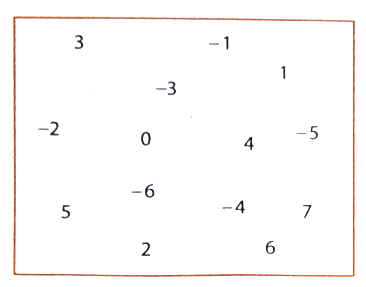
\includegraphics[width=0.9\linewidth]{6FMA46_imagens/imagem1}
    		\\ 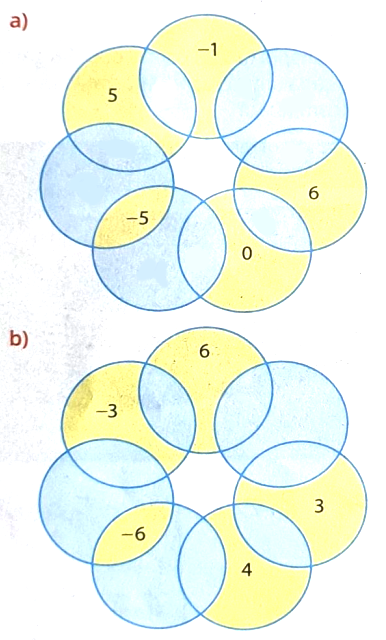
\includegraphics[width=0.9\linewidth]{6FMA46_imagens/imagem2} \\
    		\item Você sabia que $a - b = a +(-b)$ sendo $a, b \in \mathbb{Z}$? Dessa forma, -1 - 2 = -1 + (-2) = -3 e 3 -(-4) = 3 + (-(-4)) = 3 + 4 = 7. Com base nessas informações, escreva dentro de cada círculo vazio (que esteja entre dois círculos com valores inteiros) a diferença entre o maior e o menor inteiro que estiverem na mesma linha desse círculo. Complete todos os círculos vazios. \\\\
    		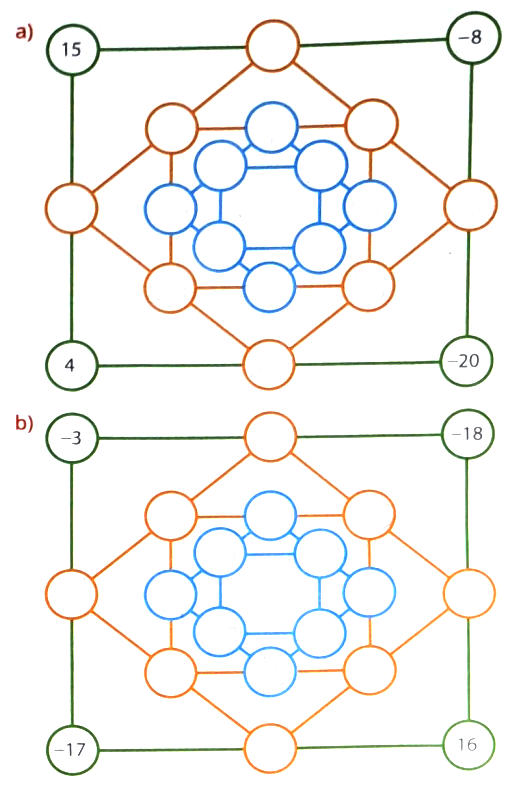
\includegraphics[width=1\linewidth]{6FMA46_imagens/imagem3} 
    		\newpage 
    		\noindent Muitos dos grandes matemáticos, em certo momento de suas vidas, depararam-se com quebra-cabeças que acabaram se transformando em teoremas. Neste laboratório estamos resolvendo, criando e pesquisando quebra-cabeças matemáticos.
    		\textsubscript{---------------------------------------------------------------------}
    		\item Distribua os números dentro dos círculos, utilizando cada um deles uma única vez, de modo que a soma de cada linha seja igual a 20.
    		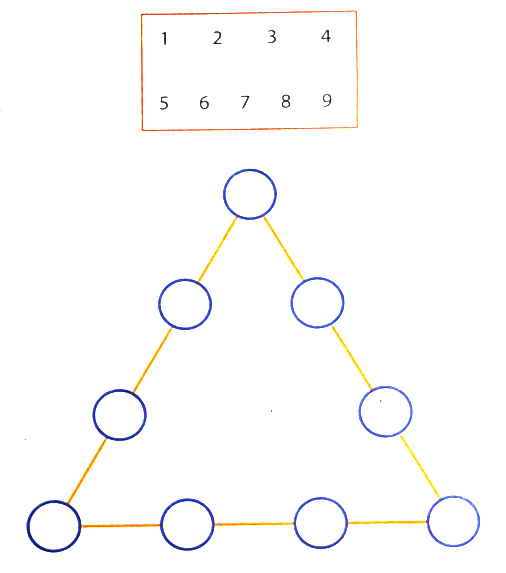
\includegraphics[width=1.1\linewidth]{6FMA46_imagens/imagem4} \\\\
    		\noindent\textbf{Agora é a sua vez} \\
    		\item Use os modelos não preenchidos para criar mais dois quebra-cabeças iguais aos do exercício 1 e mais dois iguais aos do exercício 2. Use os números que você quiser e o terceiro modelo como rascunho.
    		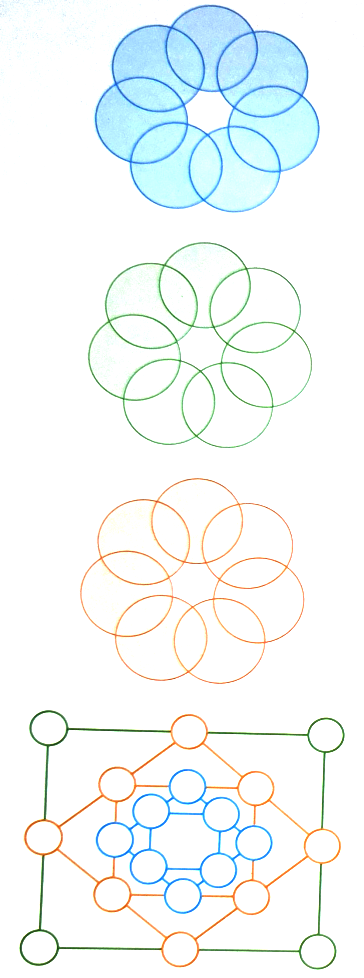
\includegraphics[width=1.1\linewidth]{6FMA46_imagens/imagem5} 
    		\newpage
    		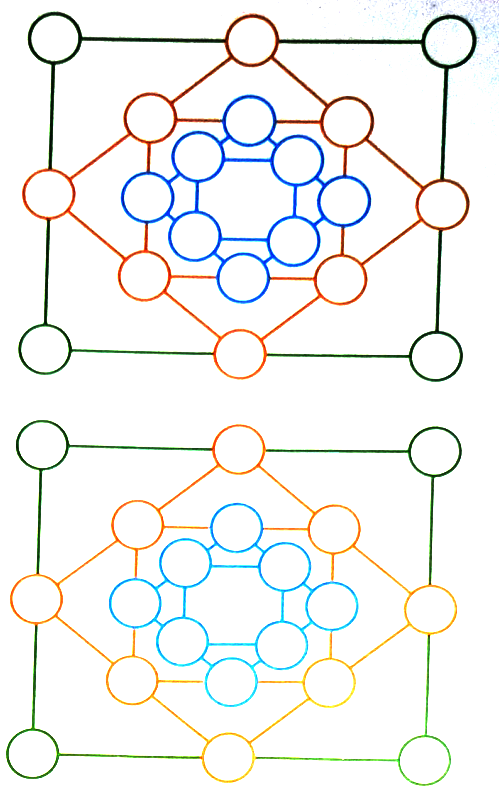
\includegraphics[width=1.1\linewidth]{6FMA46_imagens/imagem6} 
    		\\\\
    		\textbf{Pesquisa}\\\\
    		Procure em livros, revistas ou na internet outros quebra-cabeças matemáticos (Não se esqueça de colocar a resposta também.)\\\\\\\\\\\\\\\\\\\\\\\\\\\\
    		\textbf{Desafio olímpico} \\\\
    		(OBMEP) Davi estava fazendo uma conta no caderno quando sua caneta estragou e borrou quatro algarismos, como na figura. Ele se lembra que só havia algarismos ímpares na conta. Qual é a soma dos algarismos manchados? \\
    		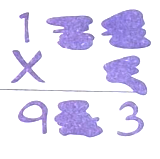
\includegraphics[width=0.6\linewidth]{6FMA46_imagens/imagem7} 
    		\\\\
    		a) 14 ~ b) 18 ~ c) 20 ~ d) 26 ~ e) 28
    	\end{enumerate}
    	$~$ \\ $~$ \\ $~$ \\ $~$ \\ $~$ \\ $~$ \\ $~$ \\ $~$ \\ $~$ \\ $~$ \\ $~$ \\ $~$ \\ $~$ \\ $~$ \\ $~$ \\ $~$ \\ $~$ \\ $~$ \\ $~$ \\ $~$ \\
	\end{multicols}
\end{document}